%% ----------------------------------------------------------------
%% Thesis.tex -- MAIN FILE (the one that you compile with LaTeX)
%% ---------------------------------------------------------------- 
% Set up the document
\documentclass[a4paper, 11pt, twoside]{Thesis}  % Use the "Thesis" style, based on the ECS Thesis style by Steve Gunn
%\graphicspath{{Figures/}}  % Location of the graphics files (set up for graphics to be in PDF format)

% Include any extra LaTeX packages required
\usepackage[square, numbers, comma]{natbib}  % Use the "Natbib" style for the references in the Bibliography
 \bibpunct{(}{)}{;}{a}{}{,}
\usepackage{verbatim}  % Needed for the "comment" environment to make LaTeX comments
\usepackage{vector}  % Allows "\bvec{}" and "\buvec{}" for "blackboard" style bold vectors in maths
\usepackage[utf8]{inputenc}
\usepackage{graphicx}
 \DeclareGraphicsExtensions{.eps,.ps}
\usepackage{overpic}
  \setlength\unitlength{1mm}
\usepackage{subfigure}
\usepackage{txfonts}
\usepackage{rotating}
\usepackage{amsmath, amssymb, amsthm,textcomp}
\usepackage{xspace}
\usepackage{multicol}
\usepackage{balance}
%\usepackage{hyperref}
%\hypersetup{urlcolor=black, colorlinks=true}  % Colours hyperlinks in blue, but this can be distracting if there are many links.
\citestyle{aa}
%% -------------------------------------------------------------------

\begin{document}
\frontmatter	  % Begin Roman style (i, ii, iii, iv...) page numbering

% Set up the Title Page 
\titleeng  {A multifrequency view of Active Galactic Nuclei}
\titlespa  {Una visi\'on multifrecuencia de N\'ucleos de Galaxias Activas}
\authors  {\texorpdfstring
            {\href{ordovas@ifca.unican.es}{Ignacio Ordov\'as Pascual}}
            {Ignacio Ordov\'as Pascual}
            }
\addresses  {\groupname\\\deptname\\\univname}  % Do not change this here, instead these must be set in the "Thesis.cls" file, please look through it instead

\date       {\today}
\subject    {}
\keywords   {}

% Title page in spanish
\maketitlespa
\newpage{\pagestyle{empty}\cleardoublepage}  

%% ----------------------------------------------------------------



\setstretch{1.3}  % It is better to have smaller font and larger line spacing than the other way round

% Define the page headers using the FancyHdr package and set up for one-sided printing
\fancyhead{}  % Clears all page headers and footers
\rhead{\thepage}  % Sets the right side header to show the page number
\lhead{}  % Clears the left side page header

\pagestyle{fancy}  % Finally, use the "fancy" page style to implement the FancyHdr headers
%% ----------------------------------------------------------------

% Declaration Page required for the Thesis, your institution may give you a different text to place here
\Declaration{

\addtocontents{toc}{\vspace{1em}}  % Add a gap in the Contents, for aesthetics

	 \large{\textbf{\tutorname}, \degreenameb,} 

	  \bigskip

          y

	  \bigskip

	  \large{\textbf{\supname}, \degreename,}\\ 

          \vspace{1.0cm}
	  
	  \large{\textbf{CERTIFICAN} ~ que la presente memoria }\\ 

          \vspace{1.0cm}
	  
	  \begin{center}
	  \large{\textbf{ \titlenamespa}} \\
          \end{center}
	  \vspace{1.0cm}
	  
	  \large{ha sido realizada por \textbf{\authornames} bajo nuestra direcci\'on. \\ 
	    Consideramos que esta memoria contiene aportaciones suficientes para construir la tesis
	    Doctoral del interesado.}

	  \vspace{2.5cm}
	  \large{En Santander, a 11 de Julio de 2018}\par % \\ \\ \\
          \bigskip
          \bigskip
          \bigskip
	  \large{\tutorname~~~~~~~~~~~~~~~~~~~~~~~~~~~~~~~~~~~~~~~~~~~~~~~~~~~ \supname} 
          \vfill
}
\cleardoublepage  % Declaration ended, now start a new page
 

% Begin the Dedication page
\pagestyle{empty}  % Page style needs to be empty for this page
\dedicatory{La dedicatoria apropiada.\ldots}

\addtocontents{toc}{\vspace{2em}}  % Add a gap in the Contents, for aesthetics
%% ----------------------------------------------------------------


% The Acknowledgements page, for thanking everyone
\acknowledgements{
\addtocontents{toc}{\vspace{1em}}  % Add a gap in the Contents, for aesthetics
% Agradecimientos

Agradecimientos

Caca

Cacacacacacacacca.
 
}
\clearpage  % End of the Acknowledgements
%% ----------------------------------------------------------------


% The Abstract Page in spanish
\addtotoc{Resumen en castellano}  % Add the "Abstract" page entry to the Contents
\abstract{
\addtocontents{toc}{\vspace{1em}}  % Add a gap in the Contents, for aesthetics

\chapter*{Resumen de la tesis en castellano}
% Resumen en castellano de la tesis
\lhead{Resumen}

\hyphenation{mo-de-ra-da-men-te re-a-li-dad mo-de-ra-do}

\section*{Objetivos de la Investigación}

Relleno.

\section*{Planteamiento y metodología}

Relleno.


\section*{Aportaciones originales}

Relleno.


\section*{Conclusiones}

Relleno.


\section*{Futuras líneas de investigación}

Relleno.




}

\cleardoublepage  % Abstract ended, start a new page
%% ----------------------------------------------------------------


% Set up the Title Page in english
\maketitleeng
\newpage{\pagestyle{empty}\cleardoublepage}

%\cleardoublepage
%% ----------------------------------------------------------------
% The "Funny Quote Page"
\pagestyle{empty}  % No headers or footers for the following pages

\null\vfill
% Now comes the "Funny Quote", written in italics
\begin{flushright}
\textit{``I am your father.''}\par
\smallskip
Lord Voldemort \\
(John Ronald Reuel Tolkien, Game of Thrones)
\end{flushright}
\bigskip
\begin{flushright}
\textit{``The problem with quotes found on internet \\
is that they are often not true.''}\par
\smallskip
Abraham Lincoln
\end{flushright}s

\vfill\vfill\vfill\vfill\vfill\vfill\null
\clearpage  % Funny Quote page ended, start a new page
%% ----------------------------------------------------------------



% The Abstract Page in english
\chapter*{Summary}
\addtotoc{Summary}  % Add the "Abstract" page entry to the Contents
\abstract{
\addtocontents{toc}{\vspace{1em}}  % Add a gap in the Contents, for aesthetics


Summary in english.
}

\clearpage  % Abstract ended, start a new page
%% ----------------------------------------------------------------

\pagestyle{fancy}  %The page style headers have been "empty" all this time, now use the "fancy" headers as defined before to bring them back


%% ----------------------------------------------------------------
\lhead{\emph{Contents}}  % Set the left side page header to "Contents"
\tableofcontents  % Write out the Table of Contents

%% ----------------------------------------------------------------
\lhead{\emph{List of Figures}}  % Set the left side page header to "List if Figures"
\listoffigures  % Write out the List of Figures

%% ----------------------------------------------------------------
\lhead{\emph{List of Tables}}  % Set the left side page header to "List of Tables"
\listoftables  % Write out the List of Tables

%% ----------------------------------------------------------------
% End of the pre-able, contents and lists of things


\mainmatter	  % Begin normal, numeric (1,2,3...) page numbering
\pagestyle{fancy}  % Return the page headers back to the "fancy" style

% Include the chapters of the thesis, as separate files
% Just uncomment the lines as you write the chapters

%Chapter 1: Introduction

\chapter{Introduction}
\label{chap:intro}
\lhead{Chapter 1. \emph{Introduction}}

During the 18th and 19th centuries, it was not clear that some of the ‘nebulas’ seen in the sky were part of our galaxy, or they were ‘islands-universes’ compound by stars \citep{kant1755}. Since the discovery in 1924 of a Cepheid variable star in M31 \citep{hubble29}, it became clear that some of them were extragalactic objects, or more precisely, they were galaxies like the Milky way. Using spectroscopic analysis, soon it became clear as well that some of the galaxies showed emission lines of highly ionized elements in the nuclei \citep{seyfert43} that cannot be explained just by the emission mechanisms of the stars, and so this emission is originated by a completely different phenomena. In some of this galaxies, this non stellar radiation completely outshines the galaxy starlight. This objects are called ‘Active Galactic Nuclei’ (AGN). 


Nowadays, it is widely accepted that the origin of this emission is due to supermassive black holes (SMBH) of $>$10$^{6}$  $\Msol$ in the centre of the active galaxy, whose immense gravitational potential is converted to emission due to very different mechanisms associated to the black hole, such as accretion of matter into the SMBH, incandescence or scattering of charged particles, among others (see Sec. \ref{sec1:em} for a more detailed explanation). The reasons to accept that the SMBH are the objects responsible of this highly energetic phenomena are various. The emission of normal or quiescent galaxies is produced almost entirely by stars, and its emission is mainly constrained between UV and IR light. Meanwhile, AGN show emission across all the electromagnetic spectrum, from the gamma rays to radio energies. This means that active galaxies emits in over twenty orders of magnitude in frequency. The luminosity of the AGN ranges from bolometric luminosities of 10$^{40}$ erg/s, comparable to the emission of quiescent galaxies (\Lbol $<$ 10$^{42}$ erg/s), to luminosities of 10$^{48}$ erg/s. The active nuclei emission frequently outshines the host galaxy starlight due to this high luminosities. Depending on the energy band observed, AGN show strong time variability of years (optical/IR), days (UV) or minutes (X-rays). The time variability measurements of the AGN emission leaves not doubt that it is originated in a compact region of the order of miliparsecs. Taking together the high luminosity of the nuclei emission and the compact region where they are originated, it is implied that AGN are objects with tremendous energy densities, only explainable by accretion into the SMBH in the core of the galaxy. 


There are evidences of that almost every galaxy harbors a SMBH in the nuclei with a mass in the range of millions to billions of solar masses \citep{magorrian98}, but as the one in the Milky Way (10$^6$ $\Msol$), not all of them are active. The host galaxy has a tight relation with its SMBH in the core of the galaxy. The \MSMBH /$\sigma$, \MSMBH/\Mhost,  \MSMBH/L$_{host}$  plots show an evidence that both quantities are very related. It has been found that there is a coevolution of the black hole and the galaxy, so AGN are considered a stage in galactic evolution that can be created by accretion or galaxy mergers. The power of the winds of the AGN stops the star formation, as this feedback crosses all the galaxy \citep{fabian12}. This means that the growth of the AGN is linked with the galaxy evolution \citep{kormendy13}.

As active galaxies are the most luminous and long lived objects in the Universe, they are visible at a large range of distances. In addition, the most distant object to the date is an AGN at z=7.085 \citep{mortlock11}, when the universe was only about a 10\% of its actual age. This also means that this object is the one closest objects in time to the Big Bang. The study of AGN therefore is a key to understand the evolution of the cosmos since the universe was very young. 


The Cosmic X-ray Background (CXRB) spectrum is the composition of the total AGN emission. From the analysis of the power law index of this spectrum, it is clear that not all of the AGNs are unobscured. The power law is harder ($\Gamma_{CXRB}\simeq$1.4 at E$<$10 keV) than an unobscured AGN ($\Gamma_{AGN}\simeq$1.9), and X-ray absorption have more effect at lower energies. In order to match models with the observations, we must introduce a fraction of absorbed AGN and highly absorbed AGN whose extinction is Compton thick (\NH$>$10$^{24}$\cm). The CXRB, using this assumption, is explained with a majority of absorbed AGN ,but to the date, this fraction of obscured sources is still unclear (\citealt{setti89}, \citealt{comastri95}). The extinction of these sources plays a major role in understanding the intrinsic properties of AGN.

All of this facts are pieces of evidences of the big importance of the study of AGN. In this thesis we work on understanding the environment of the AGN through its emission properties and the optical extinction and X-ray absorption of these objects. This is an important aspect of AGN, as there are some open questions to the date that challenges the Unified Model of AGN  (see Sec. \ref{sec1:um}). 


\section{Unified Model of AGN}
\label{sec1:um}

There is a great variety of AGN with different observational properties whose power is originated by the same mechanism, that is the accretion to the SMBH, so an Unified Model of AGN was proposed to explain this diversity (\citealt{antonucci93}, \citealt{urry95}). In this model, the observed differences between each class of AGN is dependent on the orientation. The Unified Model, schematically represented in Fig.~\ref{sec1:fig_um}, have the following components:




 \begin{figure}
 \centering
 %\includegraphics[width=8.5cm]{Chapter1_intro/umagn.ps}
 \includegraphics[width=9cm]{Chapter1_intro/umagn.ps}
 \includegraphics[width=9cm]{Chapter1_intro/agnanatomy.ps} 
    \caption{Up: Artistic representation of the Unified Model of AGN (credit: C.M. Urry and P. Padovani). Down: Skech of the componets of the Unified Model and its distance to the central SMBH (credit: K. Gebhardt webpage).}
 \label{sec1:fig_um}
 \end{figure}



\begin{enumerate}
\item \textbf{Accretion disk:} The material falling into the SMBH forms a thin disk optically thick whose size is estimated to be of $\sim$10$^{-2}$ pc. The disc emission is a multi-component black body of T$\sim$10$^{5\pm 1}$K

\item \textbf{SMBH corona:} This is where the X-ray emission is originated and it is thought to be linked to the accretion disk forming a system. The hot plasma in the corona is hit by photons from the disk. A fraction of them, due to inverse Compton scattering, is reflected in the hard X-rays. This direct relation between the corona and the accretion disk is clear in the linear relation between the hard X-rays and the UV luminosity. Other photons are radiated back to the accretion disk. This contributes to maintain the accretion disk balanced and to form the corona-accretion disk system.

\item \textbf{Boad Line Region (BLR):} This region is formed by dust-free clouds of highly ionized gas. From the difference of line ratios from the core to the wings of the broad lines, it is indicated that this region is not a thin spherical shell \citep{crenshaw86}. The material on the BLR is believed to form clouds orbiting at high velocities around the black hole. This clouds are thought to be at the far end of the accretion disk at a distance of 0.01-0.1 pc from the SMBH. The opening angle of this region is unknown to the date. This region explains the broad emission lines observed in the UV/optical spectrum with a large Doppler broadening of FWHM velocities of $>$1500 km/s. The emission of the disk ionizes this region producing the broad permitted lines in emission detected in the AGN spectrum. From line diagnostics, it is expected that its clouds are dense ($\sim$10$^9$ cm$^{-3}$) and reaching temperatures of T$\sim$20000 K. For some objects there are detected other ‘sub-regions’ of the BLR, such as an intermediate line region (ILR) and a very broad line region (VBLR).


\item \textbf{Narrow Line Region (NLR):} The narrow lines observed in the UV/optical spectrum of AGN have FWHM velocities comparable to the host galaxy bulge stellar velocity. This lines are produced by the emission of gas clouds further away from the central engine ($\sim$100 pc), and hence, with lower ionization than in the BLR and not affected by variability. The lines produced in the NLR are forbidden and permitted lines that are excited by the accretion disk emission. From line diagnostics, it is expected that the clouds are less dense (10$^{3}$ cm$^{-3}$) and cooler (T$\sim$18000K) than the BLR. There is no transition region between the BLR and the NLR, they are completely separated regions in the AGN model.


\item \textbf{Torus:}  Outside of the BLR, there is a dusty region with a toroidal geometry surrounding the black hole at a distance of $\sim$1 pc. This component is the key to explain the variations in the observed spectrum of the different AGN classes. Depending on the angle of view, covers the corona, accretion disk and BLR emission (in the case of a type-2 AGN), or gives a clear view of these central regions (type-1 AGN). More recent studies assume the dust to reside in clumps rather than being smoothly distributed. The nuclear emission is absorbed and scattered, and hence it heats the dust and re-emits it at NIR/FIR frequencies. This is not the only source of the emission at NIR/FIR, as dust also emits at these frequencies in the polar outflow of the AGN \citep{honig17}. 

\item \textbf{Radio Jet:} The jets are originated at the sub-parsec scales of the AGN and can often be traced up to distances of the order of kpc or Mpc. The radio emission is due to synchrotron emission of electrons ejected at relativistic energies in the polar direction. Large-scale jets are usually divided into FR I and FR II jets \citep{fanaroff74}. FR I jets have low luminosity ($<$10$^{41}$ erg/s) that ends in radio lobes. FR II jets have a high luminosity ($>$10$^{41}$ erg/s) collimated jet that ends in hotspots.


\end{enumerate}

The different regions in the Unified Model emmits at different wavelengths due to different emission mechanisms. In the following section we explain the different contributions to the spectral energy distribution (SED) with respect to this model.




\section{Physical mechanisms of emission}
\label{sec1:em}

We pointed out that AGN are detected in a wide range of energy ranges. In this section we list and explain the AGN emission in each of the available observational windows, and where are originated taking into account the Unified Model described in the previous section. In Fig. \ref{sec1:fig_sed} we show the complete SED of a normal AGN.


 \begin{figure}
 \centering
 \includegraphics[width=11cm]{Chapter1_intro/agnsed.ps}
    \caption{Typical SED of a few types of AGN from \cite{beckmann12}.}
 \label{sec1:fig_sed}
 \end{figure}


\begin{enumerate}

\item \textbf{Radio emission:} The radio spectrum is well described with a power law, indicating a non-thermal origin (synchrotron emission, see Sec.~\ref{sec1:syem}). There are two subclasses of active galaxies, that are Radio Loud (RL) AGN and Radio Quiet (RQ) AGN, depending on the ratio of the optical emission and the radio emission (see Sec.~\ref{sec1:class}). 

\item \textbf{IR emission:} the IR component is generally attributed to thermal emission from dust at a wide range of temperatures ($\sim$ 50 -1000 K). This is called the IR bump. The inflection at the blue side of the Bump is produced at $\sim$1 \um. This would correspond to the maximum temperature which dust could survive, that is around 1000-2000 K, depending on the composition of the dust grains. The IR bump peaks at 60 \um and falls dramatically in the submillimetre until the radio continuum. The radio emission, with respecto to this IR emission, drops in flux about 5-6 orders of magnitude for RQ AGN, or roughly 2 orders for RL AGN



\item \textbf{UV/optical emission:} The shape of the UV/continuum emission can be modeled with a multi-component black body of T$\sim$10$^{5\pm1}$K. This is feature of the SED is called the Big Blue Bump (BBB), and usually is the peak of the AGN luminosity. The relative strengths of the IR and Big Blue bumps are generally comparable, but is not the same for all AGN. Superimposed to this featureless continuum there are permitted emission lines, with full width at half-maximum (FWHM) velocities of $>$1000 km/s from the Broad line region, and both permitted and forbidden and other emission lines with FWHM velocities comparable with the ones of the stellar at the bulge. In addition, there are blends that form pseudo continuum regions originated by two elements: one is the FeII pseudo continuum, with velocities comparable to the ones of the broad lines or slightly lower, and the continuum produced the by  the high order Balmer lines. In particular there is a bump at the wavelength region of the MgII line called the Small Blue Bump, that is formed by a combination of those two blends.  

\item \textbf{X-ray emission:} The emission in the X-rays is mainly a power law emission extending from 1keV to over 100 keV. In the energy space the flux can be modeled with a power law F$_E\sim$E$^{-\Gamma}$, being the photon index around $\Gamma\sim$1.9. Below 2 keV, an emission excess is visible in the X-ray continuum (the ’soft excess’) in 30\% of AGN. The origin is not clear, but is sometimes associated to thermal emission linked to the accretion disk or collisionally-ionized diffuse gas. At energies harder than 10 keV, it is sometimes detected the presence of an exponential term that peaks around 80-300 keV and a bump that peaks at 30 keV (the ’Compton reflection hump’). This spectral feature is often explained as reflection of the direct X-ray continuum in the accretion disk or the molecular torus \citep{turner09}. For some AGN it is visible a strong emission line at 6.4 keV, that is the fluorescent Fe K$\alpha$ line.

\item \textbf{Gamma ray emission:} Blazars, a subclass of AGN, emits the majority of the bolometric luminosity above 100MeV. The spectrum of this sources is characterized by a non-thermal continuum, a flat radio spectrum and a featureless optical spectrum with strong variability and polarization.

\end{enumerate}


The main ingredient for the conversion of the gravitational energy to emission is the accretion of material into the SMBH. Comparing the bolometric luminosity of the AGN with the maximum luminosity that the SMBH can irradiate (the Eddington luminosity, L$_{Edd}$), we can estimate the accretion of the AGN (the Eddington ratio, $\lambda$), assuming normally accretion efficiencies of about $\epsilon\sim$0.1. In the literature we can find objects accreting at very low Eddington ratios ($\lambda$=10$^{-2}$-10$^{-3}$) to objects emitting at super-Eddington ratios \citep{raimundo09}.

This thesis focus more in the X-ray and UV/optical emission, so below we are explaining in a deeper way the emission mechanisms responsible of the emision at these energies. In Fig.~\ref{sec1:fig_xe} we are showing the components of the X-ray emission of an AGN. In Fig.~\ref{sec1:fig_oe} we are showing composite AGN spectra from \cite{shen16} to help to understand the intrinsic UV/optical emission of an average AGN. 


 \begin{figure}
 \centering
 \includegraphics[width=\textwidth]{Chapter1_intro/xagn.ps}
    \caption{X-ray spectrum for a normal AGN, with the different components of the X-ray emission overplotted with different colors. Figure from \cite{risaliti04}.}
 \label{sec1:fig_xe}
 \end{figure}


\subsection{Primary X-ray emission}
\label{sec1:xem}

\subsubsection{Free-free emission}
\label{sec1:ffem}

Also called Bremsstrahlung emission, this is produced when free electrons are accelerated or decelerated in the Coulomb field of an atomic ionized nuclei and radiate energy. When a charged particle approaches to other one it will be deflected, and hence it will change the movement by accelerating or decelerating. This change of momentum of the two charges will provoke the emission of a photon whose amplitude is proportional to the charge of the two interacting particles in this process. In AGN this emission could be originated in a hot ionized gas near the SMBH. The medium of the BLR could be opaque to the free-free radiation meanwhile low density nebulae are optically thin to this radiation \citep{netzer90}.

\subsubsection{Sycrotron emission}
\label{sec1:syem}

This is the radiation produced when the charged particles are accelerating at relativistic velocities in a magnetic field. The particle changes direction due to the perpendicular force. The photon emitted is proportional to the energy of the electron, the magnetic field, and the angle between those two vectors.

\subsubsection{Inverse Compton scattering}
\label{sec1:csem}

The inverse Compton scattering is the main contribution to the X-ray emission. This is produced by the interaction of low energy photons with high energy electrons, resulting in a gain of energy by the photons. The photons from the accretion disk that are emitted in the UV/optical energies interact with the electrons in the hot corona of the SMHB moving at relativistic energies. The emission of this phenomena is a power-law X-ray spectrum with a typical slope of $\Gamma$=1.9 (\citealt{caccianiga04}, \citealt{gaalbiati05}, \citealt{mateos05a}, \citealt{mateos05b}, \citealt{tozzi06}, \citealt{mateos10}, \citealt{corral11}).

\subsection{X-ray reflection}
\label{sec1:xrem}

X-ray photons at lower energies tends to be more absorbed than scattered, meanwhile photons at hard energies are more likely to be reflected. This provokes that the reflection spectrum of an AGN is a bump between 5-10 keV peaking at $\sim$30 keV, that produces a flattening of the spectral slope at hard energies.

\subsection{Fe emission line}
\label{sec1:feem}

There is often detected an emission line at 6.4 keV. This is the  Fe-K line of the transition n=2-1 for $\leq$FeXVII. The presence of this line is thought to be provoked by fluorescence in the inner part of the accretion disk. The typical EW of the line is 100 - 200 eV. The line has an asymmetrical profile with a red wing, but generally the X-ray spectra quality is not enough to show it.





\subsection{Emission in the UV/Optical range}
\label{sec1:opem}


 \begin{figure}
 \centering
 \includegraphics[width=\textwidth]{Chapter1_intro/test_shen_agn.ps}
    \caption{UV/optical QSO template from \cite{shen16}. TEMPORAL.}
 \label{sec1:fig_oe}
 \end{figure}


\subsubsection{UV/Optical continuum}
\label{sec1:coem}

When matter approaches to a massive object with a high angular momentum, it falls forming an accretion disk. The disk has annuli at many different temperatures so it is a sum of many blackbody spectra with a T$_{eff}\sim$10$^5$ K, that peakes at the UV/optical. This is the origin of the featureless blue continuum in the spectrum of an AGN. Redwards 10000 \AA, the continuum slope changes due to the emission from the IR bump originated in the torus. The emission off AGN in the UV/optical range is compound by a sum of a featureless continuum from the accretion disk, and emission lines from the NLR and the BLR. The other continuum contributions are blends of emission lines (like FeII) and bound-free pseudocontinuum of the Balmer lines, that are explained in the following section.

\subsubsection{Emission lines}
\label{sec1:liem}

The most likely source of power for the UV/optical AGN emission lines to be produced is the photoionization \citep{netzer90}. The origin of the radiation that ionizes the material is the direct UV radiation of the disk. For the broad lines there are models that separates the region where the low ionization (Balmer lines, FeII, MgII) and high ionization (Ly$_{\alpha}$, CIV, CIII]) lines are emitted. The latter are likely emitted by a dilute outflowing medium, while the low ionization broad lines come mainly from material located at the outer regions of the accretion disk \citep{netzer90}. The narrow line spectrum of type-1 and type-2 are very similar, but in some type-1 AGN there are much stronger highly ionized lines, that are emitted closer to the central engine \citep{ferguson97}.

In this thesis we are focusing more in a wavelength range redwards $\sim$2000 \AA. In this region the most conspicuous broad emission lines are, from blue to red wavelength rest-frame core of the line, MgII, \Hb and \Ha. There are other broad emission lines, but they are less prominent, such as the ones from the Balmer series of the Hydrogen, and in the infrared, the ones from the Paschen series. The FeII emission comes from the outer parts of the BLR, as they are usually found to have FWHM velocities of 0.8-1.0 times the \Hb ones \citep{osterbrock91}. They form a pseudo continuum, that is most prominent in the region of the MgII line (the Small Blue Bump, SBB), and two small regions bluewards and redwards \Hb. Nearly all broad line AGNs have optical FeII emission in their spectrum. The FeII strength is usually measured by the quantity R4570=FeII $\lambda$4570/\Hb, being  FeII $\lambda$4570 the flux of the FeII contribution measured between $\lambda$=4434-4684 \AA~and \Hb the one of the total \Hb contribution. As mentioned in \cite{veroncetty00}, this ratio is $\sim$0.1-1 for the vast majority of objects. Only a 5\% of AGN have R4570$>$1. Other pseudocontinuum from the BLR is the one formed by the stacking of the high order Balmer lines and bluewards 3646 \AA~the bound-free Balmer Continuum. This contribution appears in the SBB, along with part of the FeII emission. Normally. The forbidden narrow emission lines that are most prominent are the ones from the [OII] line, the [OIII] emission near \Hb, the [OI] line, and the doublets near \Ha from [NII] and [SII] elements. In addition, in the spectrum there are visible the narrow emission lines of the Hydrogen Balmer series.


The emission lines have the shape of a lorentzian profile. The velocity dispersion of the emitted material makes that the shape of the line is a gaussian profile due to Doppler broadening, as it is the dominant contribution to the width. For the broad emission lines, the centre of the line is displaced with respect to the rest-frame (\citealt{sulentic00}, \citealt{steinhardt12}, \citealt{gaskell13}). The narrow lines are not displaced but sometimes due to outflows it can be detected an extra blue component in addition to the rest frame narrow emission lines.  

This are the general and most prominent characteristics of AGN emission. Nevertheless, active galaxies present a great variety of spectra. The presence or absence and the relative strength of some of the features shown in this section leads to different AGN classifications.






\section{Classification of AGN}
\label{sec1:class}


Given the Unified Model mentioned in Sec. \ref{sec1:um} the observed spectra will depend on the orientation of the source with respect to the observer. The emision of AGN is detailed in  Sec. \ref{sec1:em}, but some of the features may be obscured or not present in the spectrum. This leads to a vast variety of classes of AGN. In this section we will detail the different classifications in the AGN zoo putting them in context with the Unified Model and the radiation that is detected by the observer. To help the reader to understand the differences and the variety of AGN classes we include a scheme in Fig.~\ref{sec1:fig_clas}.



 \begin{figure}
 \centering
 %\includegraphics[width=8.5cm]{Chapter1_intro/umagn.ps}
 \includegraphics[width=\textwidth]{Chapter1_intro/clasagn.ps}
    \caption{Schematic representation of the Unified model of AGN from \cite{beckmann12} and the different classification of the AGN incoming radiation depending on the viewing angle. }
 \label{sec1:fig_clas}
 \end{figure}



In the literature it can be found a wide variety of AGN classes and subclasses. This vast variety can be explained by a variation on very small number of parameters, such as orientation (see  Sec. \ref{sec1:um}), luminosity, variability, relative emission in some wavelengths windows, presence or absence of broad and narrow emission or absorption lines and host galaxy contribution. In Table \ref{sec1:tab_clas} we show some of the classes seen in the literature.

As mentioned in Sec. \ref{sec1:em}, AGN are divided into Radio Loud (RL) and Radio Quiet (RQ) based on the relative strength of the radio emission. This is based on the relative radio emission based on the radio loudness parameter R. This is the ratio of the 5 GHz flux to the optical (B-band) emission. RL AGN are the ones that the ratio R is larger than 10, and are approximately a 10 percent of the total AGN population. Radio emission for RL is between 2 and 4 orders of magnitude larger than the RQ AGN.

Other division is made in terms of the luminosity, that is the distinction between Seyfert galaxies and Quasar (QSO), to most luminous class of AGN. If the source have a magnitude in the B band higher than M$_{B}<$-21.5 mag, the AGN can be considered as a Quasar.


%\begin{table}
%\begin{center}
%
%\begin{tabular}{lll}
\begin{tiny}


\begin{table} %{| p{.10\textwidth} | p{.90\textwidth} |} 
\begin{center}
\caption{The AGN zoo: list of AGN classes.}
\begin{tabular}{lll}
\hline
Class/Acronym & Meaning & Main properties/reference\\
\hline
Quasar &Quasi-stellar radio source (originally) & Radio detection no longer required \\
Sey1 & Seyfert 1 & FWHM $\gtrsim 1000$ km s$^{-1}$ \\
Sey2 & Seyfert 2 & FWHM $\lesssim 1000$ km s$^{-1}$  \\
QSO &Quasi-stellar object & Quasar-like, non-radio source \\
QSO2 &Quasi-stellar object 2 & High power Sey2\\
RQ AGN & Radio-quiet AGN & see ref. 1\\
RL AGN & Radio-loud AGN & see ref. 1\\
Jetted AGN & & with strong relativistic jets;  see ref. 1\\
Non-jetted AGN & & without strong relativistic jets;  see ref. 1\\
Type 1 & & Sey1 and quasars\\
Type 2 & & Sey2 and QSO2\\
FR I &Fanaroff-Riley class I radio source & radio core-brightened (ref. 2)\\
FR II &Fanaroff-Riley class II radio source & radio edge-brightened (ref. 2)\\
BL Lac & BL Lacertae object & see ref. 3\\
Blazar & BL Lac and quasar & BL Lacs and FSRQs\\
\hline
BAL & Broad absorption line (quasar) & ref. 4\\
BLO &Broad-line object & FWHM $\gtrsim 1000$ km s$^{-1}$   \\
BLAGN &Broad-line AGN & FWHM $\gtrsim 1000$ km s$^{-1}$  \\
BLRG &Broad-line radio galaxy & RL Sey1 \\
CDQ & Core-dominated quasar & RL AGN, $f_{\rm core} \ge f_{\rm ext}$ (same as FSRQ)\\
CSS &Compact steep spectrum radio source & core dominated, $\alpha_{\rm r} > 0.5$ \\
CT & Compton-thick & $N_{\rm H} \ge 1.5 \times 10^{24}$ cm$^{-2}$  \\
FR 0 &Fanaroff-Riley class 0 radio source & ref. 5 \\
FSRQ &Flat-spectrum radio quasar & RL AGN, $\alpha_{\rm r} \le 0.5$  \\
GPS &Gigahertz-peaked radio source & see ref. 6\\
HBL/HSP & High-energy cutoff BL Lac/blazar &  $\nu_{\rm synch~peak} \ge 10^{15}$ Hz 
(ref. 7)\\
HEG &High-excitation galaxy & ref. 8\\
HPQ & High polarization quasar & $P_{\rm opt} \ge 3 \%$ (same as FSRQ)\\
Jet-mode & & $L_{\rm kin} \gg L_{\rm rad}$ (same as LERG); see ref. 9\\
IBL/ISP & Intermediate-energy cutoff BL Lac/blazar & $10^{14} \le \nu_{\rm synch~peak} \le 10^{15}$ Hz 
(ref. 7)\\
LINER & Low-ionization nuclear emission-line regions &  see ref. 9\\
LLAGN & Low-luminosity AGN & see ref. 10\\
LBL/LSP & Low-energy cutoff BL Lac/blazar & $\nu_{\rm synch~peak} < 10^{14}$ Hz 
(ref. 7)\\
LDQ & Lobe-dominated quasar & RL AGN, $f_{\rm core} < f_{\rm ext}$\\
LEG &Low-excitation galaxy & ref. 8\\
LPQ & Low polarization quasar & $P_{\rm opt} < 3 \%$ \\
NLAGN &Narrow-line AGN & FWHM $\lesssim 1000$ km s$^{-1}$   \\
NLRG &Narrow-line radio galaxy & RL Sey2 \\
NLS1 & Narrow-line Seyfert 1 & ref. 11 \\
OVV &Optically violently variable (quasar) & (same as FSRQ)\\
Population A/B & & ref. 12\\
Radiative-mode & & Seyferts and quasars; see ref. 9\\
RBL & Radio-selected BL Lac & BL Lac selected in the radio band \\
Sey1.5/1.8/1.9 & Seyfert 1.5, 1.8 or 1.9 & ref. 13 \\
SSRQ &Steep-spectrum radio quasar & RL AGN, $\alpha_{\rm r} > 0.5$   \\
USS & Ultra-steep spectrum source & RL AGN, $\alpha_{\rm r} > 1.0$ \\
XBL & X-ray-selected BL Lac & BL Lac selected in the X-ray band\\
XBONG & X-ray bright optically normal galaxy & AGN only in the X-ray band/weak lined AGN\\
\hline
\end{tabular}
\scriptsize Table extracted from \cite{padovani17}. The top part of the table relates to major/classical classes. The last column describes themain properties. When these are too complex, it gives a reference to the first paper, which defined the relevant class or, when preceded by ``see'', a recent paper, which gives up-to-date details on it. Reference key: 1. \cite{padovani16}; 2. \cite{fanaroff74}; 3. \cite{giommi12}; 4. \cite{weymann81}; 5. \cite{ghisellini10}; 6.\cite{odea91}; 7. \cite{padovani95}; 8. \cite{laing94}; 9. \cite{heckman14};  10. \cite{ho08};11. \cite{osterbrock85}; 12. \cite{sulentic02}; 13. \cite{osterbrock81}.

\label{sec1:tab_clas}
\end{center}
\end{table}

\end{tiny}

In this thesis we are focusing more in the classifications based on the X-ray and UV/optical wavelengths. The principal division at these energies is between type-1 and type-2 AGN. In the optical spectrum, a type-1 AGN is the one that shows broad emission lines with FWHM$\gtrsim$1000 km/s, edited in the BLR. Additionally, the optical spectrum presents narrow emission lines whose widths are comparable with the stellar velocity dispersion of the spheroidal component. The continuum from the accretion disk as it is low or not extinguished, is blue and frequently is more luminous than the host galaxy emission. Type-2 AGN show an optical spectrum that shows only narrow emission lines superimposed to the host galaxy spectrum. The broad emission lines in this case are obscured and so not detected in the spectrum. The continuum from the accretion disk is reddened and its emission is obscured as well.

The type-1 Seyfert galaxies are also divided in terms of the FWHM of the \Hb and FeII emission. When the FWHM of the broad \Hb line is less than 2000 km/s, the \Hb/[OIII]$<$3, and there is significant contribution of FeII. However, as discussed in \cite{veroncetty00} and references therein, this division is rather arbitrary. 

AGN emission features can be partially or totally outshined by stellar light from the galaxy (\citealt{severgnini03}, \citealt{georgantopoulos05}, \citealt{caccianiga07}, \citealt{caccianiga08}). Even that is normal that AGN contribution is the one that is more powerful in general, there are low luminosity AGN whose features are hard or impossible to measure. If these low luminosity sources have some level of extinction, its emission will be even harder to detect. This could make the source to be misclassified, or to be labeled as an XBONG.

In the X-rays, the Unified Model assumes that the differences between type-1 and type-2 results from the amount of absorbing gas in the line of sight. There is no consensus in the limit to divide between type-1 and type-2. From \cite{caccianiga08}, it is used the limit \NH$>$4$\times$10$^{21}$\cm \cm, that comes from the limit \Av=2 mag, that normally obscures the broad lines in the spectrum. Other studies find the limit in \NH$>$10$^{22}$\cm\citep{ueda03}, and use this more conservative limit to ensure that this extinction is intrinsic from the AGN and does not come from Galactic gas .

There is as well subdivisions in the type-1/type-2 classifications, due to the fact that there are intermediate types with detectable but weak broad emission lines. The relative strength of the broad lines with respect to the narrow lines that can not be explained simply by type-1 or type-2 provoked the need to add a subclassification. In this thesis we subclasiffy the AGN into type-1.0/1.2/1.5/1.8/1.9 following the scheme from \cite{whittle92}:

\begin{itemize}
\item \textbf{Seyfert 1}: Objects showing broad \Hb emission line and with [O III]/\Hb $<$ 0.3
\item \textbf{Seyfert 1.2:} Objects showing broad \Hb and with 0.3 $<$ [O III]/\Hb $<$ 1
\item \textbf{Seyfert 1.5:} Objects showing broad \Hb and with 1 $<$ [O III]/\Hb $<$ 4
\item \textbf{Seyfert 1.8:} Objects showing broad \Hb and with 4 $<$ [O III]/\Hb
\item \textbf{Seyfert 1.9:} Objects not showing broad \Hb, but having broad \Ha
\item \textbf{Seyfert 2:} Objects without \Ha nor \Hb broad-line emission 

\end{itemize}

This subclassification due to the relative strength of the broad lines with respect to the narrow line emission has a direct relation with the partial obscuration of the central parts of an AGN.  The strength of the broad emission, emitted in regions close to the SMBH, is partially extinged from the torus. Meanwhile, narrow emission is emitted farer away from the SMBH, less affected by obscuration.

Additionally, as mentioned in \cite{veroncetty06}, in the literature are examples of objects without UV/optical broad emission lines detected, but that they show Paschen broad emission lines in the infrared \citep{goodrich94}. This sources are classified as S1i, and this is explained because in this sources the high dust extinction make the UV/optical lines undetectable, but in the infrared, less affected by dust extinction, they can be detected. There are as well the S1p class, that do not show broad emission lines, but they are detected in the polarized spectrum (\citealt{antonucci85}, \citealt{miller90}, \citealt{tran92}).

The observed radiation of an AGN is heavily affected by the obscuration of the material in the line of sight, so a good understanding on the extinction mechanisms is hence needed in order to explain the differences in the observed spectrum (ie. in classification) of active galaxies.


\section{Absorption and obscuration}
\label{sec1:abs}


Once established the unified model of AGN, it is clear that the obscuration plays a main role in understanding the observed properties of AGN. The amount of obscuration in the line of sight will determine the classification in terms of type-1 or type-2. Understanding the absorption mechanisms in each band will help us to test the unified schemes and to recover the intrinsic properties of the active galaxies. To do so, in this section we explain the extinction models in the optical range and in the X-rays. 

The radiation emitted has to go through various materials until it reaches us. First it must cross the surrounding material of the AGN. Depending on the orientation, it will pass different quantity and density of dust and gas. As it was explained in the previous section, the emission that propagates in the radial direction of the disk, will be absorbed by the BLR and the torus and will be completely blocked. Meanwhile, the radiation that propagates outside of the torus covering angles will escape through the AGN practically unaffected. Outside of the nuclei, it will be affected by material in the interstellar medium of the host galaxy, such as dust lanes or gas clouds. Finally, it will be absorbed by the Galactic extinction. This last contribution to the incoming extinction is know and can be corrected in X-rays using the NHI Galactic maps \citep{dickey1990} and in the UV/optical assuming a measured dust-to-gas relation of the Milky Way, and thus converting \NH to \Av.

Dust grains are the main ingredient responsible of UV/optical extinction via scattering and absorption of the emitted photons. As the effect of the scattering and absorption is more effective at wavelengths comparable to dust grains size ($\lambda$=2$\times \pi \times$a, being a the size of the dust grain), its effect is higher at lower wavelengths. Depending on the dust grains, the extinction can differ. In Fig.~\ref{sec1:fig_ao} we show different extinction models and the effect with the wavelength. There is as well a feature around 2175 \AA~that is the Carbon dip, that is explained by PAHs and graphite \citep{weingartner01}. This is detected in various models and absent in others. The dust. For QSO, the extinction model that best explain the reddening curve is the one from the Small Magellanic Cloud \citep{hopkins04}, being one of the most used the one from \cite{gordon03}. The absence of the Carbon dip favours an scenario where the small grains coagulates forming bigger grains \citep{maiolino01}.


 \begin{figure}
 \centering
 \includegraphics[width=10cm]{Chapter1_intro/ext.ps}
    \caption{Different models of the ratios of dust extinction with respect to wavelength. Figure from \cite{noll05}.}
 \label{sec1:fig_ao}
 \end{figure}




One of the methods used to measure the amount of optical reddening in the source is by computing the Balmer Decrements. This consists in compare the relative strengths of emission lines, mainly \Ha and \Hb, but other times it is used H$_{\epsilon}$ or even Paschen lines, and compare with the intrinsic relative strengths. For the most used case, that is \Ha/\Hb, we assume a case B recombination and optically thin photoionized plasma \citep{osterbrock89}. The intrinsic value is normally assumed to be around 3.1 for the NLR and 3.4 for the BLR, without a clear and universally accepted value. Recent studies are finding that this value have a considerable spread (\citealt{jin12}, \citealt{schnorr16}), as it depends on the conditions of the emitting region \citep{netzer13}. Other method to estimate the extinction is fit the AGN continuum using an extinction model and an AGN template. This approach is no extent of inconvenients, as there are sources with a continuum intrinsically different than the average. There are a population of AGN whose continuum is redder than the average, and so the method can confuse intrinsically red object with a small amount of reddening in the source.



In a first order, the principal component that absorbs the X-ray photons is the gas in the line of sight, and within the gas, the hydrogen is the predominant element that contributes to obscure the X-ray emission. This is why the X-ray absorption is quantified in terms of the \NH column density. The probability for an X-ray photon to be absorbed follows Eq.\ref{sec1:eq_abs}: 

\begin{equation}\label{sec1:eq_abs}
P(E)=1-e^{(-\sigma(E) \times N_{\rm H})}
\end{equation}

Where $\sigma$(E) is a the cross section of the photoelectric absorption. The effect of the gas to the X-ray photons is higher at soft energies. In Fig.~\ref{sec1:fig_ax} we show the effects on a simple power law with different levels of gas in the line of sight.


 \begin{figure}
 \centering
 \includegraphics[width=\textwidth]{Chapter1_intro/absx.ps}
    \caption{The effect of gas absoption in the X-ray emission. Figure from the adaptation of \cite{wilman99} shown in \cite{singh13}.}
 \label{sec1:fig_ax}
 \end{figure}



According to the Unified Model, one source with significant extinction in the optical range should appear as absorbed in the X-rays and vice versa, but this is not happening for 10-20\% of the sources. This fraction of discordant AGN appears indepently of the selection method (eg. \citealt{panessa02}, \citealt{caccianiga04}, \citealt{mateos05a}, \citeyear{mateos05b}, \citealt{mainieri05}, \citealt{caccianiga08}, \citealt{mateos10}, \citealt{corral11}, \citealt{scott12}, \citealt{page12}, \citealt{merloni14}). The mismatch between optical extinction and X-ray absorption described above is observed in both optical/infrared and X-ray selected samples at all redshifts. The origin of such apparent discrepancies remain unclear, and hence so it is the validity of the unified model for such AGN.


There has been many attempts to explain the origin of the discrepancies for X-ray unabsorbed and optically type-2 AGN. For some AGN it is found that there is more dust in relation with the gas, although such cases are very rare (\citealt{caccianiga04}, \citealt{trippe10}, \citealt{huang12}, \citealt{malizia12}, \citealt{masetti12}, \citealt{mehdipour12}), so in this cases, the emission from the X-rays would arrive to us practically unaffected by the material in the line of sight, and the optical emission will be obscured. Other possibility is that the broad UV/optical lines are diluted by the host galaxy starlight, so in this case the source is classified as a type-2 AGN as there is not enough signal-to-noise to distinguish AGN features from the stellar emission. This is the case of XBONGS. In other objects, optical observations show an intrinsically high Balmer decrement for the Hydrogen broad emission lines, while the X-ray spectra show low absorption \citep{barcons03}. A dusty-ionized absorber can produce more relative absorption in the X-rays than in the optical emission \citep{della01}.


Compton-thick AGN can be misclassified as an unabsorbed type-2 AGN, since the direct X-ray emission below 10 keV is completely absorbed and we would only detect scattered nuclear radiation (\citealt{braito03}, \citealt{akylas09}, \citealt{braito11}, \citealt{malizia12}), which might be mistaken by direct emission. This emission is about 1-3\% of the total X-ray emission (\citealt{gilli01}, \citealt{comastri04}, \citealt{georgantopoulos11a}), therefore comparing it to the luminosity at other energies (eg. the [OIII] line) can unveil if the source is a compton thick or not. Scattered nuclear radiation would have a lower power law index as well. The EW of the Fe line at 6.4 keV would be high as well due to the relative difference between the strength of the line and the scattered nuclear radiation.


High gas-to-dust ratios could be a possible answer to high absorbed AGN in the X-rays but showing low or not extinction at UV/optical energies . The gas-to-dust ratios can increase due to dust sublimation close to the central X-ray source \citep{granato97}. Other explanation is that dust grains are biased to be bigger in the environment of AGN, more specifically small grains of dust coagulates forming larger grains \citep{maiolino01}, an explanation more plausible than the destruction of small grains in favour of larger grains, especially given that the PAHs from the Carbon dip at 2175 \AA~is not normally present in AGNs \citep{hopkins04}. Eclipsing material coming from the dust-free BLR can as well act as an additional absorption of the X-ray photons leaving UV/optical photons less affected. As the angle of aperture of the BLR is not known, nor if is similar in all AGNs, this could be a valid scenario to explain this sources. 

An independent explanation without having to invoke to non standard physics or obscuring material is that there is variability in the sources. If the optical and X-ray data has been taken at different dates, we can not discard that the discrepancies are originated by eclipses of gas and/or dusty clouds in the line of sight. The clumpy structure model of the BLR and the torus would be compatible with this explanation.  In fact, there are reports in the literature of changing look sources (\citealt{lamassa15}, \citealt{miniutti14}). Even considering variability with simultaneous optical and X-ray observations, there are sources whose classification in these energies are discordant (\citealt{corral05}, \citealt{bianchi08}, \citeyear{bianchi12}).



\section{Aims of this thesis}
\label{sec1:aim}

Describe the aims of the papers in this thesis.

Summarizing, along this work we will tackle the following issues:

\begin{enumerate}
\item One

\item Two

\item Three

\end{enumerate}

 % Introduction

\chapter{Instrumentation} % Write in your own chapter title
\label{chap:ins}
\lhead{Chapter 2. \emph{Instrumentation}} % Write in your own chapter title to set the page header

In Chap.~\ref{chap:ins} it was explained with detail the emission of AGN and its classification, derived from a great variety of spectral energy distributions. This fact makes the selection of an unbiased, uniform and complete sample of AGN an extremely difficult task. In order to perform a proper selection of active galaxies it is needed to understand the limits of each wavelength range.  

AGN were in first place detected at radio frequencies being called them Quasi Stellar Radio sources (and after, Quasars or QSO), but only a small fraction of objects emits strongly in the radio band. In the optical band it is where the maximum of emission of the AGN is, optical surveys provide large samples of AGN, but the selection techniques dramatically misses reddened objects and even host galaxy dominated ones. Infrared selection techniques are the most efficient ones to detect sources that are highly obscured and missed in the rest of the spectral bands, but this works for high luminosity sources, as it is needed to distinguish between the host IR emission and the contribution from the dust heated from the AGN.

In this thesis we used an X-ray selection based on the 2-10 keV energies. This band is sensible to X-ray absorption up to the Compton Thick limit (\NH $\sim$10$^{24}$ cm$^{-2}$). This AGN are found in the X-rays surveys identifying the counterparts in the optical for the X-ray sources, by cross-correlation of catalogs or by dedicated observations of the sources.

The selection used in this thesis is from the wide-angle (44.43 sq. degree) Bright Ultra-hard XMM-Newton Survey \citep{mateos12}. This is a flux limited ($f_{\rm 4.5-10\,keV}\geq$ 6$\times 10^{-14}$ erg s$^{-1}$ cm$^{-2}$) hard X-ray selected (4.5-10 keV) sample using the XMM-Newton observatory. The BUXS survey and the sample used are described in detail in Chap.~\ref{chap:buxs}.

This chapter will explain the instrumentation used to detect the active galaxies in the X-rays using XMM-Newton in Sec.~\ref{sec2:xr} and in the optical in Sec.~\ref{sec2:tel}, and more precisely using long-slit spectra form dedicated observations (Sec.~\ref{sec2:otel}) and fiber spectra from public surveys (Sec.~\ref{sec2:sdss}).

\section{X-ray observations}
\label{sec2:xr}

The atmosphere of the Earth is completely opaque to photons of certain energy as seen in Fig.~\ref{sec2:atm}. For some of the wavelength bands, the detectors must be at a certain altitude in order to detect its radiation. Optical emission can be detected from instruments located at the ground, as well fro some infrared energy windows. But in order to collect data from X-ray emission it is needed to place detectors in rockets or space observatories. 

 \begin{figure}
 \centering
 \includegraphics[width=\textwidth]{Chapter2_data/opac.ps}
 \includegraphics[width=\textwidth]{Chapter2_data/trans.ps}
    \caption{Top: Opacity of the atmosphere in terms of the observed wavelength (credit: NASA). Bottom: Altitude in kilometers in order to observe each wavelength range (credit: Thomson Higher Education 2007). }
 \label{sec2:atm}
 \end{figure}
 
In this thesis the X-ray data that is used comes from the X-ray Multi-Mirror satellite XMM-Newton. This is one of the four 'Cornerstone' missions defined in the Horizon 2000 Programme of the European Space Agency (ESA). 


 %\includegraphics[width=10cm]{Chapter2_data/opac.ps}




\subsection{XMM-Newton}
\label{sec2:xmm}

The spacecraft XMM-Newton was launched by an Ariane 504 from Kourou, French Guiana on 10 December 1999. The satellite is orbiting in a elliptical orbit around the Earth, with an inclination of 40$^{o}$, being the apogee at a distance between 99000 and 115000 km and the perigee between 6000 and 22000 km of altitude. The spacecraft takes 48 hours to complete an orbit.

The observatory XMM-Newton carries three scientific instruments, that are the European Photon Imaging Camera (EPIC;  \citealt{turner01}, \citealt{struder01}, see Sec.~\ref{sec2:epic}) the Reflection Grating Spectrometer (RGS; \citealt{denherder01}, see Sec.~\ref{sec2:rgs}) and the Optical Monitor telescope (OM; \citealt{mason01}, see Sec.~\ref{sec2:om}) that allows simultaneous optical and X-ray observations. In Fig.~\ref{sec2:xmmsch} we show a sketch of the XMM-Newton spacecraft.

 \begin{figure}
 \centering
 \includegraphics[width=\textwidth]{Chapter2_data/xmm.ps}
    \caption{Diagram of the XMM-Newton spacecraft (credit: ESA).}
 \label{sec2:xmmsch}
 \end{figure}
 

The three X-rays telescopes are build with 58 Wolter I grazing-incidence mirrors, being the largest mirrors of 70 cm of diameter. They are nested in coaxial and cofocal configuration with a grazing angle of 30'. The focal length of these telescopes is 7.5 m. This configuration allows that the instruments can achieve a an effective area of $\sim$ 1500 cm$^{2}$ over a wide energy range (0.1-15 keV), in particular at energies close to the rest frame Fe K$\alpha$ line.


\subsubsection{European Photon Imaging Camera (EPIC)}
\label{sec2:epic}


The European Photon Imaging Camera (EPIC) are Charge-Coupled Device cameras (CCD) that can register extremely weak X-ray radiation and can detect flux variation in the range of microseconds. these advanced Charge-Coupled Device cameras (CCD) are capable of detecting rapid variations in intensity in the range of $\sim$0.001 seconds.


They are located at the prime focus of each of the three telescopes. The EPIC camera have the following detectors, two Metal Oxide Semi-conductor (EPIC-MOS; \citealt{turner01}) and one EPIC-pn \citep{struder01}. In front of the detector, it is located a filter wheel.

\begin{itemize}

\item The EPIC-MOS consists on two sets of CCDs sensible in the 0.1-15 keV energy range, with a moderate spectral energy resolution of E/$\Delta$E=20-50. Each EPIC-MOS camera consist on a mosaic of 7 CCDs where each CCD is 600 $\times$ 600 pixels. Every single CCD have a size of 10.9' $\times$ 10.9', so the total Field of View of the MOS camera is 33' $\times$ 33'.

\item There is only one unit of the EPIC-pn camera. This one is a mosaic of  12 CCDs (64 X 200 pixels each), with a FOV of 12.6' $\times$ 4.4' each one, to obtain a total FOV of 27.5' $\times$ 27.5'. As the EPIC-MOS cameras, this unit is sensible to the energy range of 0.1-15 keV with the same spectral resolution of E/$\Delta$E=20-50.

\end{itemize}


\subsubsection{Reflection Grating Spectrometer (RGS)}
\label{sec2:rgs}


In two of the telescopes, roughly a 40 per cent of the incoming radiation is reflected to a secondary focus, where the Reflection Grating Spectrometers (RGS) are located. Those two RGS allows high resolution (E/$\Delta$E=100-500) for the soft X-ray energy range of 0.3 to 2.1 keV. The objective is to detect K-shell transitions of elements such as carbon, nitrogen, oxygen, neon, magnesium, and silicon and the L-shell transitions of iron. 

\subsubsection{Optical Monitor}
\label{sec2:om}


The last instrument onboard is the Optical Monitor (OM), that is a 30 cm Ritchey-Chretien telescope that works on the wavelength range of 1800-6500 \AA. It can collect images of the same regions as the X-ray telescope simultaneously with a FOV of $\sim$ 17' and $\sim$ 1'' of spatial resolution. The filters available are listed in Table~\ref{tab2:om}.

\begin{table}
\begin{center}
\caption{Filters available for the Optical Monitor.}
\begin{tabular}{|c|c|c|c|c|c|}
\hline
Name & $\lambda_{eff}^{(a)}$ & $\lambda_{max}^{(b)}$ &  FWHM  & PSF$_{\rm FWHM}$  & Peak mag \\ 
   &  (\AA) & (\AA) &  (\AA)  & (‘')  & (mag) \\ 
\hline
V	 & 5407 & 5230 & 684 & 	1.35 & 19.0   \\ \hline
B	 & 4334 & 3980 & 976 & 	1.39 & 19.7   \\ \hline
U	 & 3472 & 3270 & 810 & 	1.55 & 19.5   \\ \hline
UVW1	 & 2905 & 2680 & 620	 & 2.0 & 19.3   \\ \hline
UVM2	 & 2298 & 2210 & 439	 & 1.8 & 18.3   \\ \hline
UVW2	 & 2070 & 2000 & 500	 & 1.98 & 17.6  \\ \hline
WHITE$^{(c)}$ &   &   &   &  & 22.2 \\ 
\hline
\end{tabular}

 (a): Effective wavelength; (b): Wavelength of maximum transmission; (c): An ‘'open'' filter.

\label{tab2:om}
\end{center}
\end{table}



\section{Ground based telescopes}
\label{sec2:tel}


In order to classify and identify all the X-ray sources, optical observations are made. Some of the optical counterparts comes from the SDSS public archive. Others are made using follow up observations of the X-ray sources by submitting a proposal to optical telescopes.

In Sec.~\ref{sec2:otel} we show in detail the optical telescopes used to acquire the optical spectra for the X-ray sources.


\subsection{Long Slit spectra from optical telescopes}
\label{sec2:otel}


\subsubsection{VLT/X-Shooter}
\label{sec2:xsh}

The Very Large Telescope (VLT) is operated by the European Southern Observatory (ESO) at Paranal Observatory in the Atacama Desert of Chile at 2635 m above sea level. It consists of four individual telescopes (UT1:Antu, UT2:Kueyen, UT3:Melipal, UT4:Yepun), each one with a diameter of the primary mirror of 8.2 m. The instrument X-Shooter, whose detailed description can be found in \cite{vernet11}, is placed on the Cassegrain focus of the second telescope, UT2:Kueyen. In Fig.~\ref{sec2:xshsch} we show an sketch of X-Shooter. This instrument consist in a combination of 3 echelle spectrographs that provides simultaneous UV-to-NIR spectroscopy (3000-25000 \AA) with intermediate spectral resolution (R$\sim$4000-17000, depending on wavelength and slit width). The incident light is divided in three different paths through two dichorics, each one reaching a different echelle spectrograph. This is conducted using two dichorics, the first with a cut off od 5595 \AA~and the second for 10240 \AA. One arm is for the UV light (UVB:3000-5595 \AA), other for the optical (VIS:5595-10240 \AA), and the last one for the near infrared (NIR:10240-24800 \AA). Additionally UVB and and VIS optical paths incorporate an Atmospheric Dispersion Corrector (ADC) that allows to compensate the effects of differential atmospheric refraction. This allows to not to be restricted to orient the slit to the parallactic angle, as it will correct the refraction wavelength dependent slit losses independently from the airmass and the orientation of the slit. The effect on the infrared is low, so no NIR ADC is used in X-Shooter.

In this thesis we used VTL/X-Shooter for a detailed study of two AGN (See Chap.~\ref{chap:xsh}). The information setup about the used slit is shown in Table \ref{tab2:xsh}. All the slits have a fixed length of 11''.


 \begin{figure}
 \centering
 \includegraphics[width=\textwidth]{Chapter2_data/xsh.ps}
    \caption{Schematic overview of VLT/X-Shooter (credit: ESO).}
 \label{sec2:xshsch}
 \end{figure}
 

\begin{table}
\begin{center}
\caption{Used X-Shooter setup for the objects in this thesis.}
\begin{tabular}{|c|c|c|c|}
\hline
Arm & Slit Width & R  & Sampling  \\
      &   (‘')   &     ($\lambda$/$\Delta\lambda$) & (pix/FWHM) \\ \hline
UVB & 1.0 & 5100 & 6.3 \\ \hline
VIS  &  0.9 & 8800 & 6.0 \\ \hline
NIR   &  0.9 & 5100 & 6.3 \\ 
\hline
\end{tabular}
\label{tab2:xsh}
\end{center}	
\end{table}



\subsubsection{VLT/FORS2}
\label{sec2:fors}

The instrument FOcal Reducer/low dispersion Spectrograph 2 (FORS2) an instrument installed at the VLT telescope Antu (UT1), in the cassegrain focus. It can be used with multiple modes such as imaging, polarimetry, and spectroscopy. In this last one, there are available various spectroscopic modes, that are a long slit spectroscopy, moveable slitlets, and an spectroscopic mask mode. In this thesis we only used the long slit spectroscopy mode (LSS).

The nine slits available in LSS mode have widths between 0.3'' and 2.5''. The slit width is not variable. The wavelength range in FORS2 is between 3300 and 11000 \AA, with an spectral reslution of R=260-2600 depending on the grism (see Table~\ref{tab2:fors}).

\begin{table}
\begin{center}
\caption{VLT/FORS2 setup for long slit spectroscopy.}
\begin{tabular}{|c|c|c|c|c|c|}
\hline
Grism name  & $\lambda_c$  & Wavelength range & Dispersion & R \\
 + ESO number & (\AA)  & (\AA) & (\AA/mm)  & (foe 1'' slit) \\ \hline
GRIS 600B+22	 & 4650 & 3300-6210 & 50  &  780  \\ \hline
GRIS 300V+10 (1) & 5900 & 3300-(6600) & 112  & 	440 \\ \hline
GRIS 300V+10	 & 5900 & 4450-8650 & 12  &  440 \\ \hline
GRIS 300I+11	 & 8600 & 6000-11000 & 	108  &  660 \\ \hline
GRIS 150I+27 (1) & 7200 & 3300-(6500) & 225  & 260  \\ \hline
GRIS 150I+27 (1)	 & 7200 & 4450-(8800) & 230  &  260 \\ \hline
GRIS 150I+27	 & 7200 & 6000-11000 & 	230  &  260 \\ \hline
GRIS 1400V+18 & 5200 & 	4560-5860 & 20.8  &  2100 \\ \hline
GRIS 1200B+97 & 4350 & 	3660-5110 & 24.0  &  1420 \\ \hline
GRIS 1200R+93 & 6500 & 	5750-7310 & 25.0  & 2140  \\ \hline
GRIS 1028z+29 & 8600 & 7730-9480 & 28.3  &  2560 \\ \hline
GRIS 600RI+19 & 6780 & 5120-8450 & 55  & 1000  \\ \hline
GRIS 600z+23 & 9010 & 7370-10700 & 54  & 1260   \\ 
\hline
\end{tabular}

(1) If used without or with the listed order separation filter, the orders will overlap above the given wavelength.
\label{tab2:fors}
\end{center}	
\end{table}



\subsubsection{GTC/OSIRIS}
\label{sec2:gtc}

The Gran Telescopio CANARIAS (GTC) is the largest optical telescope to date. The primary mirror of the GTC is formed by a set of 36 hexagonal mirrors that forms a mosaic of a mirror of 10.4 m of diameter. This telescope is placed at the Roque de los Muchachos Observatory on the island of La Palma, Spain, at 2396 m above sea level. The GTC was built by the public company GRANTECAN S.A., that also operates it.

The instrument that is used in this thesis for long slit spectroscopy is OSIRIS (Optical System for Imaging and low-Intermediate-Resolution Integrated Spectroscopy), located in the Nasmyth-B focus. This instrument uses slits with widths ranging from 0.4'' to 10'', and with a length of 7.4' for all of them. Ositis is composed by two CCDs. The objects that are being observed are centered in the coordinate X=200 of the CCD2 in order to minimize the cosmetic effects that could affect the spectrum, as CCD1 have more artifacts than CCD2. Osiris can operate with resolutions between R=300 to R=2500, covering wavelength ranges between 3650 and 10500 \AA, depending on the grism or volume-phased holographic gratings (VPHs) used (see Table~\ref{tab2:osiris} for details).


\begin{table}
\begin{center}
\caption{GTC/OSIRIS setup for long slit spectroscopy.}
\begin{tabular}{|c|c|c|c|c|c|c|}
\hline
ID &  $\lambda_c$ (\AA) & $\lambda_{range}$ (\AA) & D (\AA/pix) & R & Peak Efficiency & Type \\ \hline
R300B  & 4405 & 3600 -7200 & 4.96 & 360 & 70\% & Grism  \\ \hline
R300R  & 6635 & 4800 - 10000 & 7.74 & 348 & 70\% & Grism  \\ \hline
R500B & 4745	  & 3600 - 7200 & 3.54 & 537	 & 68\%  & Grism  \\ \hline
R500R	 & 7165 & 4800 - 10000 & 4.88 & 587 & 67\% & Grism  \\ \hline
R1000B & 5455 & 3630 - 7500 & 2.12 & 1018 & 65\% & Grism  \\ \hline
R1000R & 7430 & 5100 - 10000 & 2.62 & 1122 & 65\% & Grism  \\ \hline
R2000B & 4755 & 3950 - 5700 & 0.86 & 2165 & 87\% & VPH  \\ \hline
R2500U & 3975 & 3440 - 4610 & 0.62 & 2555 & 70\% & VPH  \\ \hline
R2500V & 5185 & 4500 - 6000 & 0.80 & 2515 & 80\% & VPH  \\ \hline
R2500R & 6560 & 5575 - 7685 & 1.04 & 2475 & 80\% & VPH  \\ \hline
R2500I	 & 8650 & 7330 - 10000 & 1.36 & 2503 & 80\% & VPH  \\
\hline
\end{tabular}
\label{tab2:osiris}
\end{center}
\end{table}



\subsubsection{TNG/DOLORES}
\label{sec2:tng}

Another telescope that is used for the followup of the sources is the Telescopio Galileo Galilei (TNG), a 3.58 m optical telescope placed at the Roque de los Muchachos Observatory on the island of La Palma, Spain. TNG is operated by the 'Fundacion Galileo Galilei, with is financed by the Istituto Nazionale di Astrofisica (INAF)

For the long slit spectroscopy, we used the Device Optimized for the LOw RESolution (DOLORES, or LRS), that is placed at the at one of the Nasmyth focus of the TNG. This instrument provides low resolution spectroscopy with R=600-6000, depending on the grism used (details of each grism are shown in Table~\ref{tab2:lrs}). With LRS we can acquire spectrum in the wavelength range of from 3000 to 10073 \AA. The detector have a field of view of 8.6' $\times$ 8.6'. The slits available have widths between 0.7'' and 5.0''.

\begin{table}

\caption{TNG/DOLORES setup for long slit spectroscopy.}
\begin{center}
\begin{tabular}{|c|c|c|c|c|c|}
\hline
Name & Disp . & $\lambda_{min}$ & $\lambda_{c}$ & $\lambda_{max}$ & R  \\ 
  & (\AA/pix) & (\AA) & (\AA) & (\AA) & (for 1'' slit)  \\ \hline
LR-B	 & 2.52	 & 3000 & 5850 & 8430 & 585 \\ \hline
LR-R	 & 2.61	 & 4470 & 7400 & 10073 & 714 \\ \hline
V390	 & 0.26 & 3634 & 3900 & 4166 & 3766 \\ \hline
V486	 & 0.20 & 4612 & 4725 & 4838 & 5953 \\ \hline
V510	 & 0.22 & 4875 & 5100 & 5325 & 5950 \\ \hline
V589	 & 0.27 & 5619 & 5895 & 6171 & 5502 \\ \hline
V656	 & 0.32 & 6232 & 6560 & 6888 & 5248 \\ \hline	
V860	 & 0.44 & 8149 & 8600 & 9051 & 4000 \\ \hline
VHRV	 & 0.95 & 4752 & 5725 & 6698 & 1527 \\ \hline	
VHRR	 & 0.70 & 6238 & 7000 & 7717 & 2513 \\ \hline
VHRI	 & 0.68 & 7433 & 8130 & 8826 & 3035 \\ 
\hline
\end{tabular}
\label{tab2:lrs}
\end{center}
\end{table}


\subsubsection{WHT/ISIS}
\label{sec2:isis}

Other telescope that is used in this thesis is the 4.2 m William Herschel Telescope (WHT), that is part of the Isaac Newton Group of Telescopes (ING) situated at the Roque de los Muchachos Observatory at La Palma island, Spain. The ING is operated by the Particle Physics And Astronomy Research Council (PPARC) of the United Kingdom, the Nederlandse Organisatie voor Wetenschappelijk Onderzoek (NWO) of the Netherlands and the Instituto de Astrofísica de Canarias (IAC) of Spain.

Spectroscopy with the WHT is conducted using the Intermediate dispersion Spectrograph and Imaging System (ISIS), mounted at the Cassegrain focus. The instrument consists on two arms, so a dichroic divides the incoming light in two beams with the dividing wavelength at roughly 5300 \AA. The blue arm works with a wavelength range between 3000 and 6000 \AA, and the red arm between 5000 and 10000 \AA. The spectral resolutions are between R=500 and R=12000 for the blue arm, and between R=900 and R=10000 for the red arm (see Table~\ref{tab2:isisb} and Table~\ref{tab2:isisr} for details for each arm). ISIS uses slits with a length of 4' and widths between 0.14'' and 22.6''.


\begin{table}
\begin{center}
\caption{WHT/ISIS blue arm setup for long slit spectroscopy.}
\begin{tabular}{|c|c|c|c|c|c|}
\hline
Grating & Blaze & Spectral range (\AA) & Dispersion (\AA/pix) & Resol. with a 1'' slit (\AA) & R \\ \hline
R158B	 & 3600 & 6635 & 1.62 & 7.81  & 512 \\ \hline
R300B	 & 4000 & 3539 & 0.86 & 4.1  & 976 \\ \hline
R600B	 & 3900 & 1825 & 0.45 & 2.02 & 1980  \\ \hline
R1200B & 4000 & 940 & 0.23 & 0.85 & 4706 \\ \hline
H2400B & Holo  & 442 & 0.11 & 0.35 & 11429  \\ 
\hline
\end{tabular}
\label{tab2:isisb}
\end{center}
\end{table}


\begin{table}
\begin{center}
\caption{WHT/ISIS red arm setup for long slit spectroscopy.}
\begin{tabular}{|c|c|c|c|c|c|}
\hline
Grating & Blaze & Spectral range (\AA) & Dispersion (\AA/pix) & Resol. with a 1'' slit (Å) & R \\ \hline
R158R	 & 6500 & 7530 & 1.81 & 7.7 & 909 \\ \hline
R316R	 & 6500 & 3858 & 0.93 & 3.8 & 1842 \\ \hline
R600R	 & 7000 & 2054 & 0.49 & 1.81 & 3867 \\ \hline
R1200R & 7200 & 1055 & 0.26 & 0.75 & 9333 \\ 
\hline
\end{tabular}
\label{tab2:isisr}
%\caption{Used X-Shooter setup for the objects in this thesis.}
\end{center}
\end{table}


\subsubsection{WHT/ACAM}
\label{sec2:acam}

With the WHT, we used another instrument for spectroscopy, that is the auxiliary-port camera ACAM. This instrument is mounted at a  Cassegrain focus and can be used not only for low resolution spectroscopy, but for broad-band imaging, narrow-band imaging as well. ACAM works with a spectral range of 3500-9400 \AA. The dispersor is a VPH grating, modelled to deliver the spectral resolution R on axis (this is, with the target near the middle of the slit) that we show it in Table~\ref{tab2:acam}. ACAM have slit widths between 0.5’’ and 10’’.

\begin{table}
\begin{center}
\caption{R for WHT/ACAM long slit spectroscopy calculated with different slit widths.}
\begin{tabular}{|c|c|c|c|}
\hline
Wavelength & 0.75 ‘’ & 1.0 ‘’ & 1.25 ‘’ \\ \hline
3800 \AA & 390 & 290 & 230 \\ \hline
5650 \AA & 580 & 430 & 350 \\ \hline
7500 \AA & 770 & 570 & 460 \\ 
\hline
\end{tabular}
\label{tab2:acam}
%\caption{Used X-Shooter setup for the objects in this thesis.}
\end{center}
\end{table}

\subsubsection{NOT/ALFOSC}
\label{sec2:not}

The 2.5 m Nordic Optical Telescope (NOT) is used for optical follow up. It is located at Roque de los Muchachos, La Palma, Canarias, Spain, and was constructed and is operated by the Nordic Optical Telescope Scientific Association (NOTSA). 

The instrument used to obtain the spectra is the Andalucia Faint Object Spectrograph and Camera (ALFOSC). The instrument have horizontal slits with widths ranging from 0.4’’ to 40.0‘’ and 6.3’ length (except the 1.0’’ and 1.8’’ slits, that have a length of 5.3’), and vertical long slits with widths from 0.5’’ to 10.0’’ and a length of 5.3’. The dispersor elements are listed in Table~\ref{tab2:not}.

\begin{table}
\begin{center}
\caption{NOT/ALFOSC setup for long slit spectroscopy.}
\begin{tabular}{|c|c|c|c|c|c|}
\hline
Grism & Grating & $\lambda_{blaze}$ & $\lambda_{c}$ & Dispersion & R \\ 
  & (rules/mm)  & (\AA) & (\AA) & (\AA) & (for 1'' slit) \\ \hline
3 & 400 & 3900 & 4320 & 2.3 & 350  \\ \hline
4 & 300 & 4800 & 5800 & 3.3  &  360 \\ \hline
5 & 300 & 6500 & 7000 & 3.5  & 415  \\ \hline
6 & 600 & 3900 & 4020 & 1.5  & 490  \\ \hline
7 & 600 & 5300 & 5260 & 1.7  & 650  \\ \hline
8 & 600 & 6500 & 7030 & 1.4  &  1000 \\ \hline
10 & 150 & 3800 & 3870 & 5.9  & 105  \\ \hline
11 & 200 & 5200 & 5000 & 4.6  &  190 \\ \hline
12 & 75 & 7300 & 6930 & 12  &   95 \\ \hline
14 & 600 & 4288 & 4630 & 1.6  &  600 \\ \hline
16 & 1000 & 4069 & 4280 & 0.86  &  1000	 \\ \hline
17 & 2400 VPH  & - & 6580 & 0.26  & 5000  \\ \hline
18 & 1086 VPH  & - & 4360 & 0.93  &  1000 \\ \hline
19 & 823 VPH   & - & 5640 & 1.2  & 970  \\ \hline
20 & 484 VPH   & - & 7850 & 2.2  &  770 \\ 
\hline
\end{tabular}
\label{tab2:not}
%\caption{Used X-Shooter setup for the objects in this thesis.}
\end{center}
\end{table}
%http://www.not.iac.es/instruments/alfosc/grisms/


\subsubsection{NTT/EFOSC2}
\label{sec2:ntt}

Other telescope used from the observatory at La Silla, at an altitude of 2400 metre in the southern part of the chilean Atacama desert, is the ESO New Technology Telescope (NTT), that is an altitude-azimuth Richey-Chretien telescope with a diameter of its primary mirror of 3.58 m.

We used the ESO Faint Object Spectrograph and Camera v.2 (EFOSC2) to obtain low resolution spectroscopy for the optical followup of the sources. This telescope have a great variety of grisms, with wavelength ranges from 3200 to 11000 \AA. The resolution varies from R=600 to R=14000, as seen in Table~\ref{tab2:ntt}.

\begin{table}
\begin{center}
\caption{NTT/EFOSC2 setup for long slit spectroscopy.}
\begin{tabular}{|c|c|c|c|c|c|c|}
\hline
Grisms & Wavelength  & Grating  & Blaze angle & Dispersion  & R & Resolution  \\ 
  & range  & (gr/mm)   & (\AA) & (\AA/pix)   &  & FWHM (\AA)  \\ \hline
  Gr 01 & 3185-10940  & 100   &    4500   & 6.66 & 676 & 48.0  \\ \hline
  Gr 02 & 5100-11000  & 100    &   6700  &  6.6 & 1015 & 49.6  \\ \hline
  Gr 03  & 3050-6100   & 400    &   3900   & 1.5 & 2600 & 11.6  \\ \hline
  Gr 04  & 4085-7520   & 360    &   4700   & 1.68 &  2798 & 12.6  \\ \hline
  Gr 05  & 5200-9350   & 300    &   6700  &  2.06 &  3252 & 15.4  \\ \hline
  Gr 06  & 3860-8070   & 300   &    5000  &  2.06 &  2427 & 15.5  \\ \hline
  Gr 07  & 3270-5240   & 600    &   3800  &  0.96 &  3958 & 7.4   \\ \hline
  Gr 08 &  4320-6360  &  600    &   5300  &  0.99 &  5354 & 7.4   \\ \hline
  Gr 09  & 4700-6770   & 600   &    5600  &  1.0  &  5600 & 7.6   \\ \hline
  Gr 10  & 6280-8200   & 600   &    6500  &  0.95  & 6842 & 7.1   \\ \hline
  Gr 11  & 3380-7520   & 300    &   4000 &   2.04  & 1961 & 15.8  \\ \hline
  Gr 12  & 6015-10320  & 300   &    7900  &  2.12 &  3726 & 16.0  \\ \hline
  Gr 13  & 3685-9315   & 236    &   4400   & 2.77 &  1588 & 21.2  \\ \hline
  Gr 14  & 3095-5085   & 600   &    4000  &  0.93  & 4301 & 7.0   \\ \hline
  Gr 15  & 6895-8765   & 600    &   8300  &  0.86  & 9651 & 6.5   \\ \hline
  Gr 16  & 6015-10320 &  300    &   7900  &  2.12  & 3726 & 16.0  \\ \hline
  Gr 17  & 6895-8765  &  600     &  8300  &  0.92  & 9022 & 6.5   \\ \hline
  Gr 18  & 4700-6770 & 600    &   5600 &   1.0  &  5600 & 7.6   \\ \hline
  Gr 19  & 4441-5114 & 1557   &   4777 &   0.34  & 14050  & 1.5   \\ \hline
   Gr 20  & 6047-7147 & 1070 & 6597 & 0.55 & 11995 & 2.0   \\ 
  \hline
\end{tabular}

\label{tab2:ntt}
%\caption{Used X-Shooter setup for the objects in this thesis.}
\end{center}
\end{table}

\subsection{Fiber spectra from SDSS survey}
\label{sec2:sdss}



In order to identify the optical counterparts of the X-ray sources, we used as well the public spectra from the Sloan Digital Sky Survey (SDSS) until the Data Release 14 \citep{abolfathi18}. The SDSS is an international collaboration that uses a dedicated 2.5m modified Ritchey-Chrétien altitude-azimuth telescope placed at the Apache Point Observatory, New Mexico, USA, at 2788 m above the sea level.

The telescope can work on imaging and spectroscopic mode. To do so, the camera at the Cassegrain focus must be changed to the corresponding instrument. To obtain optical spectra, SDSS uses plates that are drilled specifically to observe the chosen celestial objects of interest for each sky field observed. Each hole in the plate is connected a fiber to drive the incoming radiation to the two spectrographs mounted on the image rotator.

For this thesis we used the data collected using two different spectrographs, the old SDSS-I/II spectrograph and the most modern one, the Baryon Oscillation Spectroscopic Survey (BOSS) spectrograph.  In Fig.~\ref{sec2:bosssch} we show a sketch of the instrument.

 \begin{figure}
 \centering
 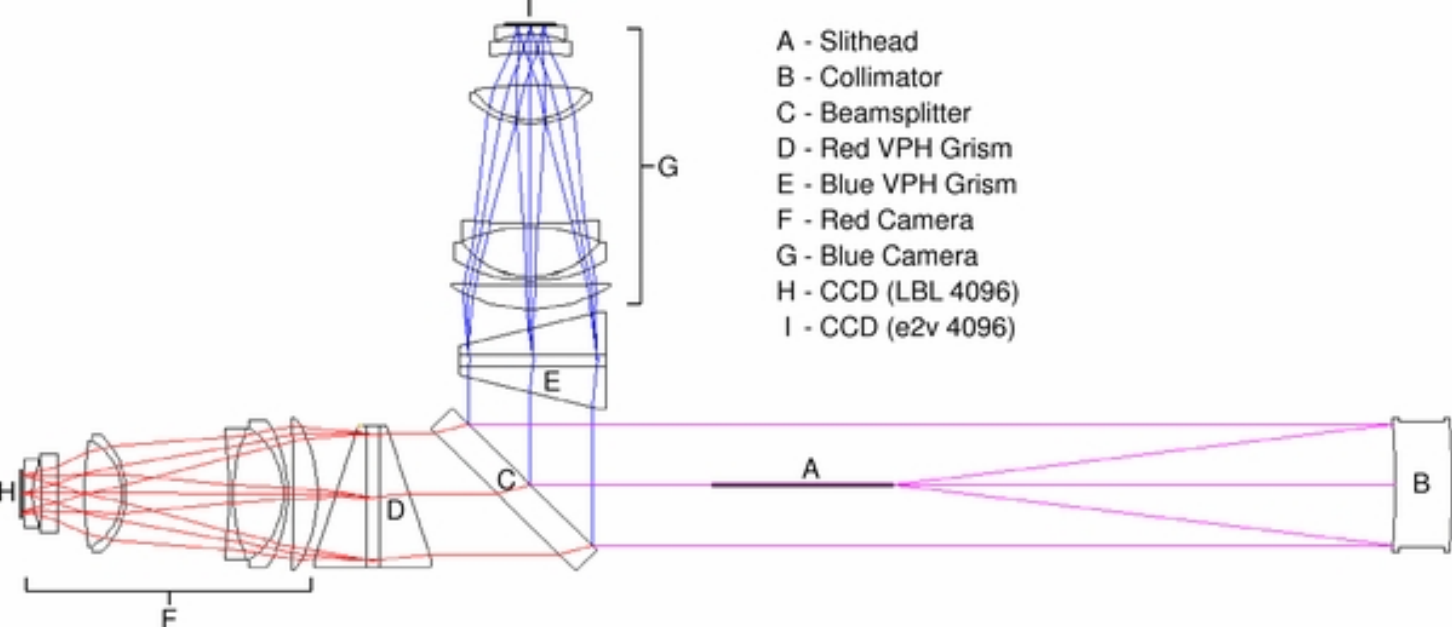
\includegraphics[width=\textwidth]{Chapter2_data/boss.ps}
    \caption{Diagram of the BOSS instrument (credit: ESA).}
 \label{sec2:bosssch}
 \end{figure}

\subsubsection{SDSS-I/II Spectrograph}
\label{sec2:sdss_spec}


The first spectroscopic instrument from SDSS acquired spectra from 640 positions in the sky for each aluminium plate. The optical fibers carry the incoming light from the focal plane to slitheads attached to the cartridge. The light is driven to two spectrographs one to cover the blue wavelength range of 3800 to 6100 \AA~and the other for the red part of the spectra, from 5900 to 9100 \AA. The beam is splitted with a dichroic with the dividing wavelength at around 6000  \AA. Each spectrograph collects the radiation with one SITe/Tektronix 2048 $\times$ 2048 CCD for each arm. This setup allows to have a resolution ranging from 1850 to 2200 for the spectral range of 3900-9100 \AA.


\subsubsection{BOSS Spectrograph}
\label{sec2:boss}

The BOSS spectrograph were a redesign of the originals SDSS spectrographs and were rebuilt from them. In this case, the aluminium plates are drilled with 1000 holes corresponding to a determinate position in the sky, and the fibers have a diameter of 2’’. The new instrument can provide a spectra with a wavelength range of 3600-10400 \AA. The light for each object is splitted with a dichroic at roughly 6000 \AA. The light is then carried to two arms, the blue channel has a wavelength range of 3700-6000 \AA~with an spectral resolution ranging from R=1560 to R=2270, at 3700 and 6000 \AA, respectively. The red arm have a resolution ranging from R=1850 to R=2650, at 6000 and 9000, respectively. 

 % Instrumentation and data origin

%Chapter 3

\chapter{The BUXS Sample} % Write in your own chapter title
\label{chap:buxs}
\lhead{Chapter 3. \emph{The BUXS Sample}} % Write in your own chapter title to set the page header

         
%- BUXS y submuestra de tipos-1
%- Ajustes y extracción rayos-X
%- Ajustes del contínuo óptico/NIR de AGN
% - Ajustes de líneas

            - SEDs
\section{Sample definition}
\label{sec3:samp}
In this section we explain how the BUXS sample is selected and the final selection, optical completeness.

\section{X-ray modeling}
\label{sec3:xray}

In this section we explain how the X-ray data were treated. We explain that we combine all the available observations. After that sources were extracted using info from other part. Apart from that we explain that the spectral modelig were based on XMMFITCAT. This is how we select the best model, how we calculate the parameters as the luminosity and nh and how compute errors.

\section{Optical spectral continuum modeling}
\label{sec3:op}

In this section we explain the reduction of an optical spectrum. We may distinguish between echelle of xshooter and long slit spectra from other telescopes, as one was analyzed with STARLIGHT and power laws, and the other with SHERPA and combinations of templates.

Apart from that we explain the ways of fitting the optical spectra. We talk about STARLIGHT for the xshooter, and sherpa for the BUXS sample.

The general model is AGN plus SMC extinction and additive host galaxy model. For some objects where we have data in the high order f the Balmer lines and higher, it is necessary to introduce FeII and Balmer Continuum emission, so we describe all the components here.


\section{Optical emision lines fits}
\label{sec3:lines}

Here we describe the H$_{\rm \alpha}$, H$_{\rm \beta}$ and MgII line fit models. The NLR uses the same width in velocity. We use the FWHM and flux as free parameters.


\section{Subsample used in this thesis}
\label{sec3:sample}

Here we give details of the data used in this thesis. In the following chapters we explain more precisely the subsamples. % The BUXS sample and methods




\chapter{Analysis of XSHOOTER} % Write in your own chapter title
\label{chap:seds}

\lhead{Chapter 4. \emph{Analysis of XSHOOTER}}

\section{Motivation}
None


 % Xshooter 2 objectss



\chapter{Analysis of BUXS sample}
\label{chap:type1}
\lhead{Chapter 5. \emph{Analysis of BUXS sample}}

We study the obscuration of type-1 AGN by comparing the optical extinction and the X-ray absorption.


\section{Sample definition}
\label{sec5:samp}

We describe here that we select all objects that show at least one broad line in their optical spectrum, that is ranging from type-1.0 to type-1.8/9, often grouped with type-2 AGN. We use only the redshift range of z=0.05-1 to measure in a robust way the X-ray obscuration.

\section{X-ray and optical}

\subsection{X-ray properties}

Here we explain the X-ray spectral fitting of the type-1 sources. In this section we also examine the percentage of X-ray absorbed sources and compare it with other samples. We test the evolution of the X-ray luminosity with the  fraction of absorbed sources.


\subsection{Optical spectrum fits}

We describe the model used to fit the optical spectrum. This allows us to measure the optical extinction of the sources in terms of Av. We can compare here the Av range of other selections and the fraction of sources not optically obscured.

\subsubsection{SED Av vs spectrum Av}

We compare this estimations with the ones from the SED analysis.

\subsubsection{Balmer decrement Av vs spectrum Av}

We compare this estimations with the ones where H$_{\alpha}$ and H$_{\beta}$ are available. We test if there is an intrinsic H$_{\alpha}$/H$_{\beta}$ ratio, or it depends on the conditions on the BLR.



\section{Subdivision in Seyfert subclases}

We study the change in parameters such as Av, NH, etc with the Seyfert subclass. We also check with different redshifts if there is an evolution or not.


\section{Optical extinction versus X-ray absorption}

We plot the Av vs NH, and we compute the fraction of sources that follows the Galactic dust-to-gas relation, the ones that are more dusty and the ones that have more gas.

\section{Dust-to-gas ratio}

Plotting the dust-to-gas ratio versus the luminosity or redshift to test if there is any dependence in between those quantities.



\section{Bolometric luminosity and Bolometric correction}

Here we test if the relations between the Bolometric luminosity based on the optical spectrum and the luminosity of the X-rays is compatible with the ones reported in other studies.



\section{Conclusions of the statistical study}

We summarize the main differences that this complete sample of type-1 AGN have with other optical or X-ray selected samples. We explain this differences with context with the unified model of AGN and with the latest explanations in the literature of optical extinction and X-ray absorption.





  % Type-1 BUXS sample

% Chapter 6

\chapter{Conclusions and future work} % Write in your own chapter title
\label{conc}
\lhead{Chapter 6. \emph{Conclusions and future work}} % Write in your own chapter title to set the page header


\section{Conclusions of this thesis}

\subsection{Detailed analysis of two X-ray unabsorbed type-2 objects}

We determined that the discordant optical and X-ray sources are not a physical family, as the origin of the discordance can be very different.

\subsection{Optical extinction and X-ray absorption of a complete type-1 sample}

The preliminar results obtained is that using a complete sample of X-ray selected type-1 AGN at hard energies we can detect objects with high levels of obscuration in the optical and in the X-rays. The majority of the sources follow the Galactic relation, but there are a significant fraction of discordant sources.


\section{Future work}

Here we explain possible studies that can be derived from this work, that could not be studied in this thesis.




 % Conclusions and future work


%% ----------------------------------------------------------------
% Now begin the Appendices, including them as separate files
\addtocontents{toc}{\vspace{2em}} % Add a gap in the Contents, for aesthetics

\appendix % Cue to tell LaTeX that the following 'chapters' are Appendices

% Appendix A

\chapter{Tables }
\label{app:tables}
\lhead{Appendix A. \emph{Tables of data}}

Along this appendix a table is presented 

%\begin{table}
%\begin{tabular}[ht]{cc}
%\input{Appendices/iras00182.tab}   &   \input{Appendices/irasF00235.tab} \\
%\end{tabular}
%\end{table}
	% Appendix Title

\addtocontents{toc}{\vspace{2em}}  % Add a gap in the Contents, for aesthetics
\backmatter


%% ----------------------------------------------------------------
%\addtocontents{toc}{\vspace{2em}} % Add a gap in the References, for aesthetics


\label{References}
\lhead{\emph{References}}  % Change the left side page header to "Bibliography"
\begin{small}
\bibliographystyle{astron}  % Use the "unsrtnat" BibTeX style for formatting the Bibliography
\bibliography{../hlirgs}  % The references (bibliography) information are stored in the file named "Bibliography.bib"
\end{small}

\end{document}  % The End
%% ----------------------------------------------------------------